\documentclass[a4paper]{article}

\usepackage[margin=1.9cm]{geometry}
\usepackage{fontspec}
\usepackage[catalan]{babel}

\usepackage[hidelinks]{hyperref}
\usepackage{amsmath}
\usepackage{amsfonts}

\usepackage{multirow}

% For figures
\usepackage{float}
\usepackage{tikz}
\usepackage{tikz-dimline}
\usepackage{subcaption}

\pgfplotsset{compat=1.14}
\usetikzlibrary{patterns}

\setlength{\parindent}{0pt}
\setlength{\parskip}{0.7em}
\def\arraystretch{1.5}
\def\imgS{0.42\textwidth}

\title{\textsc{Pràctica 2} \\
	\normalsize Aplicació del mètode dels elements finits a l'anàlisi d'una peça prismàtica}

\author{Joan Marcè \and Iñigo Moreno \and Esteve Tarragó}
\date{}


\begin{document}
\maketitle

\section{Introducció}
\subsection{Objectiu}

L'objectiu de la pràctica és realitzar un anàlisi mitjançant el mètode dels elements finits d'una reixa d'embornal metà\l.lica insta\l.lada als accessos d'una nau industrial on hi ha trànsit de vehicles pesats.

\subsection{Dades del problema}
\subsubsection{Condicions del muntatge}
El conjunt a analitzar té 2 parts principals: marc inferior i reixa abatible. El marc inferior està aferrat a l'obra civil i, per tant, és una peça fixa.

La reixa abatible és una peça articulada al marc inferior mitjançant 2 perns. En condicions de servei, la reixa abatible està tancada i recolza sobre el marc inferior. Cal destacar que existeix un petit joc entre les 2 parts del conjunt per tal de permetre i facilitar el tancament de la reixa.

\subsubsection{Geometria}
La reixa abatible a analitzar està formada per un marc, 3 barres longitudinals i 2 orelles d'articulació. A la \autoref{fig:planol} es presenta un dibuix amb les dimensions bàsiques de la reixa.

\begin{figure}[H]
	\centering
	
	\begin{tikzpicture}[scale=0.15]
		% Draw the rectangle
		\filldraw[rounded corners, gray, draw=black] (0,0) -- (65, 0) -- (65, 35) -- (62.5, 35) -- (62.5, 30) -- 
			(2.5, 30) -- (2.5, 35) -- (0, 35) -- cycle;
		\foreach \i in {1,...,4} 
			\draw[fill=white, rounded corners] (2.5,{1.5*\i + (\i - 1)*5.625}) rectangle (62.5, {\i*(5.625+1.5)});
			
		% Draw cotes
		\dimline[extension start length=-4.5cm,
			extension end   length=-4.5cm,
			extension start style={black,thin},
			extension end   style={black,thin}
		]{(2.5, -3)}{(62.5,-3)}{$600$};
		\dimline[extension start length=-6cm,
			extension end   length=-6cm,
			extension start style={black,thin},
			extension end   style={black,thin}
		]{(0,-6)}{(65,-6)}{$630$};
		\dimline[extension start length=4.5cm,
			extension end   length=4.5cm,
			extension start style={black, thin},
			extension end   style={black, thin}
		]{(-4.5,0)}{(-4.5,30)}{$300$};
		\dimline[extension start length=-6cm,
			extension end length=-6cm,
			extension start style={black, thin},
			extension end   style={black, thin},
			line style={arrows=dimline reverse-dimline reverse},
			label style={below=0.8ex}
		]{(68.5, 7.125)}{(68.5,8.625)}{$15$};
		
	\end{tikzpicture}
	\caption{Plànol de la reixa (\emph{mm})}
	\label{fig:planol}
\end{figure}

Com que l'objectiu és analitzar una peça prismàtica, es modelitzarà una barra longitudinal amb les següents dimensions principals (L = 600, b = 15 i h = 40 mm)

\subsection{Material}

La reixa d'embornal està fabricada amb fosa nodular o de grafit esteroïdal (material dúctil). Les característiques del material són les següents:

\begin{table}[H]
	\centering
	\begin{tabular}{|l|c|r|}
		\hline
		\textbf{Característica} & \textbf{Símbol} & \textbf{Fosa nodular FG 38-17} \\
		\hline
		Tensió de ruptura & $f_u$ & 380 MPa \\
		Tensió del límit elàstic & $f_y$ & 235 MPa \\
		Mòdul elàstic o de Young & $E$ & 172000 MPa \\
		Coeficient de Poisson & $\nu$ & 0,275 \\
		\hline
	\end{tabular}
\end{table}

\subsection{Càrrega}
La càrrega màxima que suporta la reixa (P) correspon a la situació en que un grup de rodes d'un vehicle pesat està totalment recolzat sobre la reixa. En aquesta situació, la reixa suporta una massa de 5t.

Com a hipòtesi, es considera que tots els punts de la reixa estan sotmesos a una mateixa càrrega repartida (q), calculada respecte l'àrea neta de la reixa (àrea total menys àrea dels forats) de valor $A_{neta} = 630 \ cm^2$. Es negligeix el pes propi de la reixa.

\section{Qüestions prèvies}
\subsection{Definiu les condicions de contorn de la barra a modelitzar a la part 1}

Com a condicions de contorn es té que la barra està unida pels dos extrems tot i que un d'ells pot lliscar. En aquest cas el costat que romandrà fix serà l'esquerra pel que els desplaçaments del costat esquerra ser

\subsection{Calculeu la càrrega repartida (q)}

La pressió que s'exerceix sobre la reixa serà el pes d'una roda del vehicle (5t) entre l'àrea neta, pel que:
$$
P = \frac{m \cdot g}{A_{neta}} = \frac{5\cdot10^3 \cdot 9,81}{630 \cdot 100} = 0,779\ \frac{N}{mm^2}
$$

Així doncs la càrrega $q$ serà la pressió exercida per l'amplada de la barra pel que:
$$
q = \frac{P}{b} = 0,779 \cdot 15 = \boldsymbol{11,67 \ \frac{N}{mm}} 
$$

\pagebreak
\section{Part I: Simulació amb l'element finit plane 182}
\subsection{Anàlisi d'un model amb una malla poc refinada amb 4 elements i 10 elements en longitud (4x10 = 40 elements finits)}

\textbf{Anàlisi de la deformada i del desplaçament vertical màxim ($\delta_{y, \max}$)}
\begin{figure}[H]
	\begin{subfigure}{\imgS}
		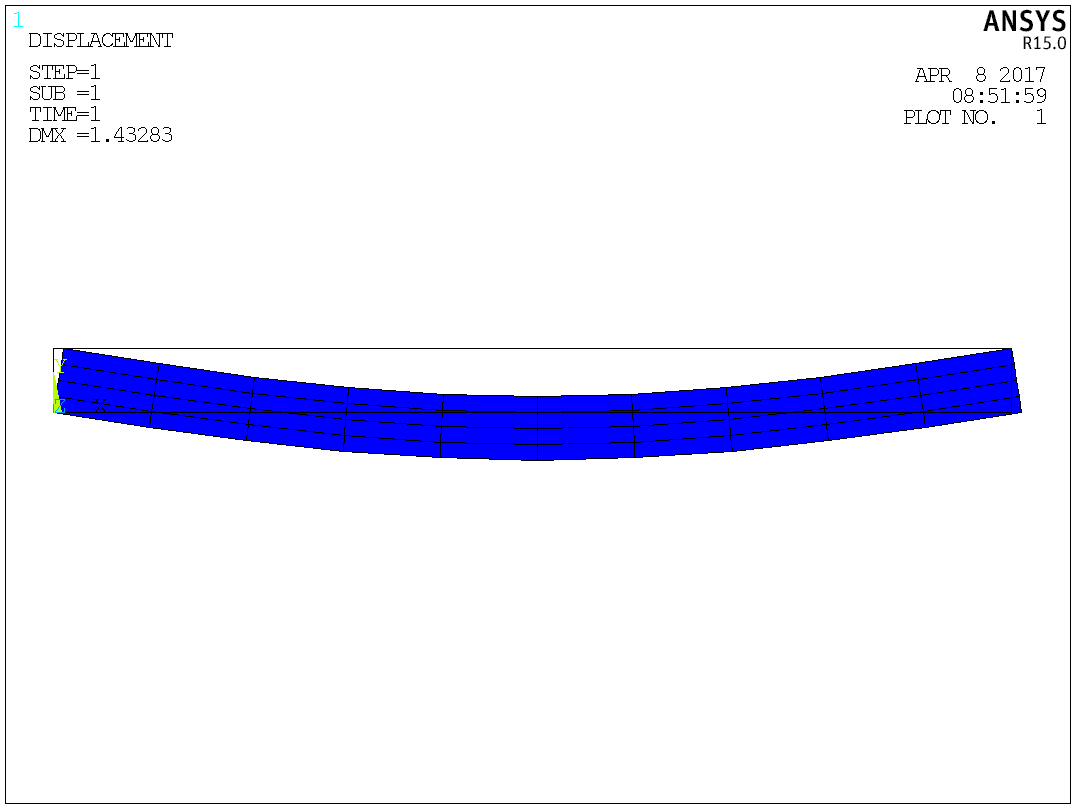
\includegraphics[width=\textwidth]{images/40_deformed}
		\caption{Deformació}
		\label{fig:40_deformed}
	\end{subfigure}
	\hfill
	\begin{subfigure}{\imgS}
		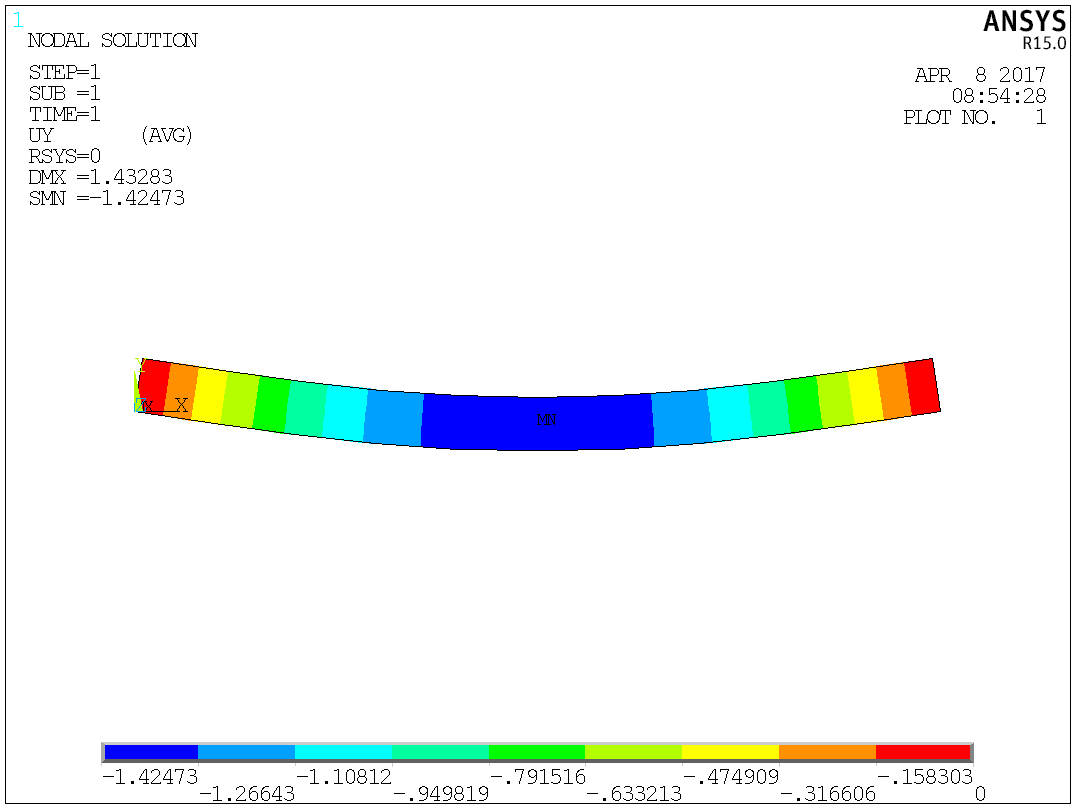
\includegraphics[width=\textwidth]{images/40_UY}
		\caption{Mapa de desplaçaments verticals UY}
		\label{fig:40_UY}
	\end{subfigure}
	\caption{Resultats del desplaçament}
	\label{fig:40_displacement}
\end{figure}

Com es pot observar a la \autoref{fig:40_UY} hi ha un desplaçament màxim de $\delta_{y, \max} = 1,42 mm$ situat al punt mig de la peça.

\textbf{Anàlisi de les tensions normals ($\sigma_x$)}
\begin{figure}[H]
	\begin{subfigure}{\imgS}
		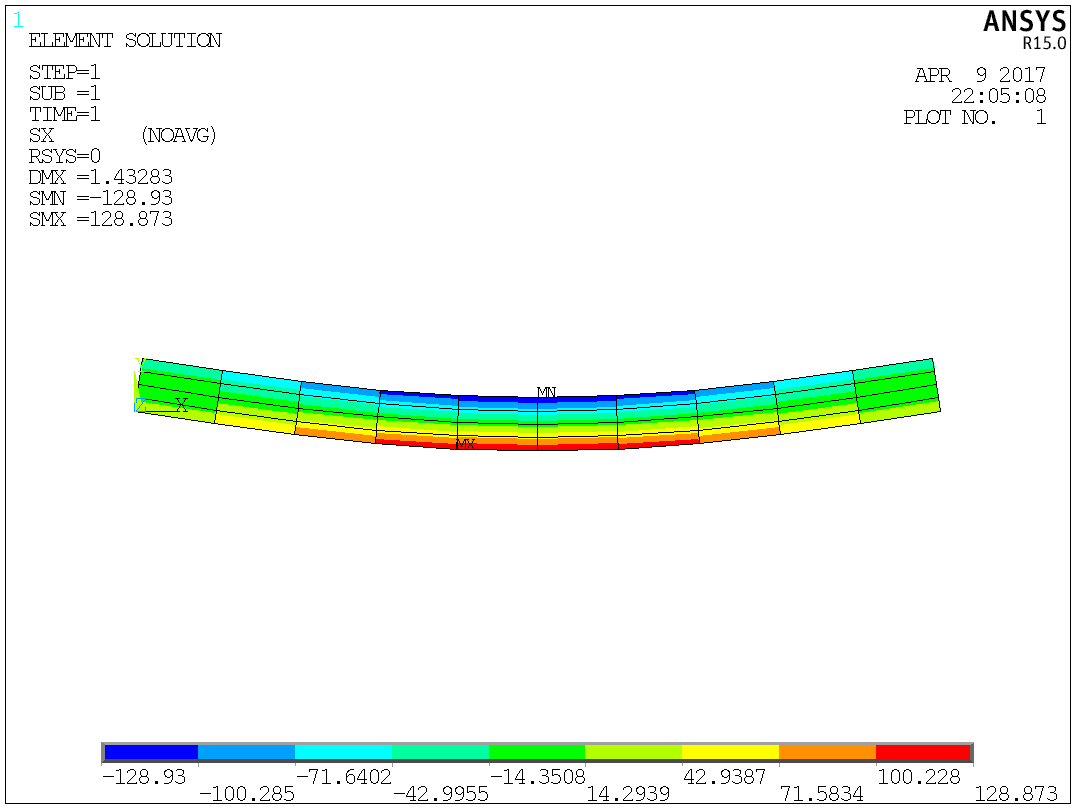
\includegraphics[width=\textwidth]{images/40_stress}
		\caption{Mapa de tensions normals {$\sigma_x$}}
		\label{fig:40_stress}
	\end{subfigure}
	\hfill
	\begin{subfigure}{\imgS}
		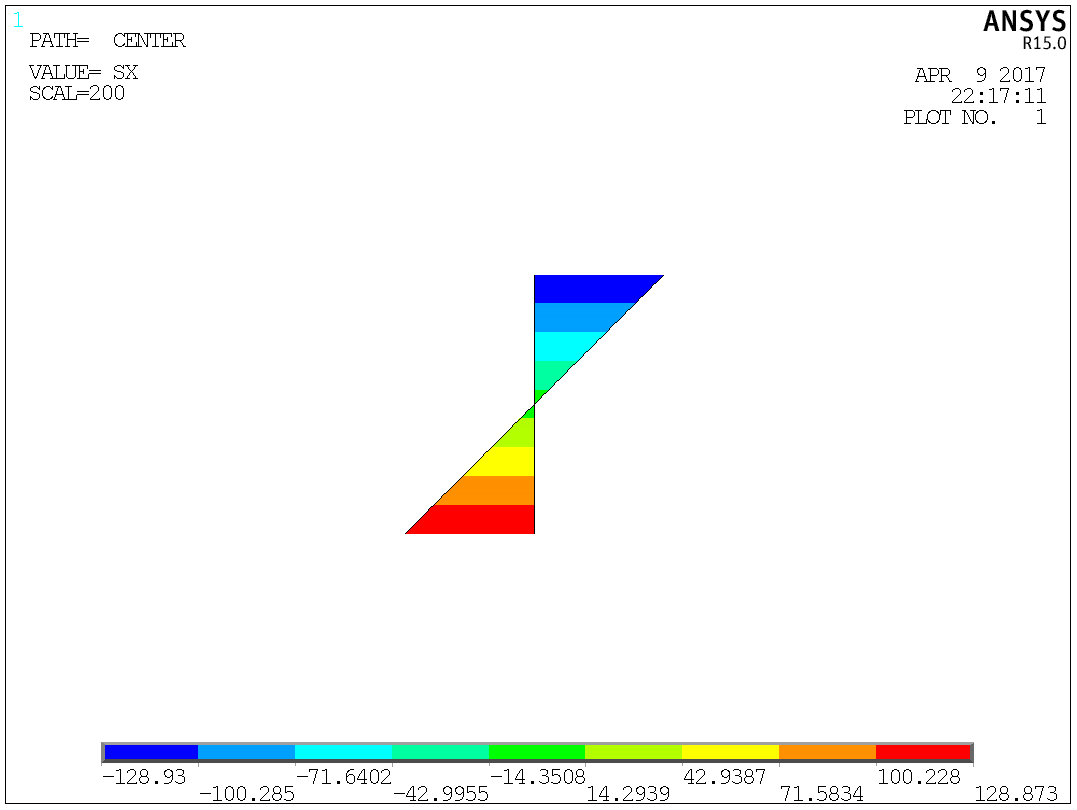
\includegraphics[width=\textwidth]{images/40_stress_path}
		\caption{Distribució de tensions normals a la secció (\emph{path})}
		\label{fig:40_stress_path}
	\end{subfigure}
	\caption{Resultats de les tensions normals}
	\label{fig:40_stress_results}
\end{figure}

Pel que fa a les tensions normals $\sigma_x$ els valors màxims i mínims també es troben al centre de la peça amb un valor de $\sigma_{x,\max+} = 128.86 MPa$ i $\sigma_{x,\max-} = -128.86 MPa$.

\pagebreak
\textbf{Anàlisi de les tensions tangencials ($\tau_{xy}$)}
\begin{figure}[H]
	\begin{subfigure}[t]{\imgS}
		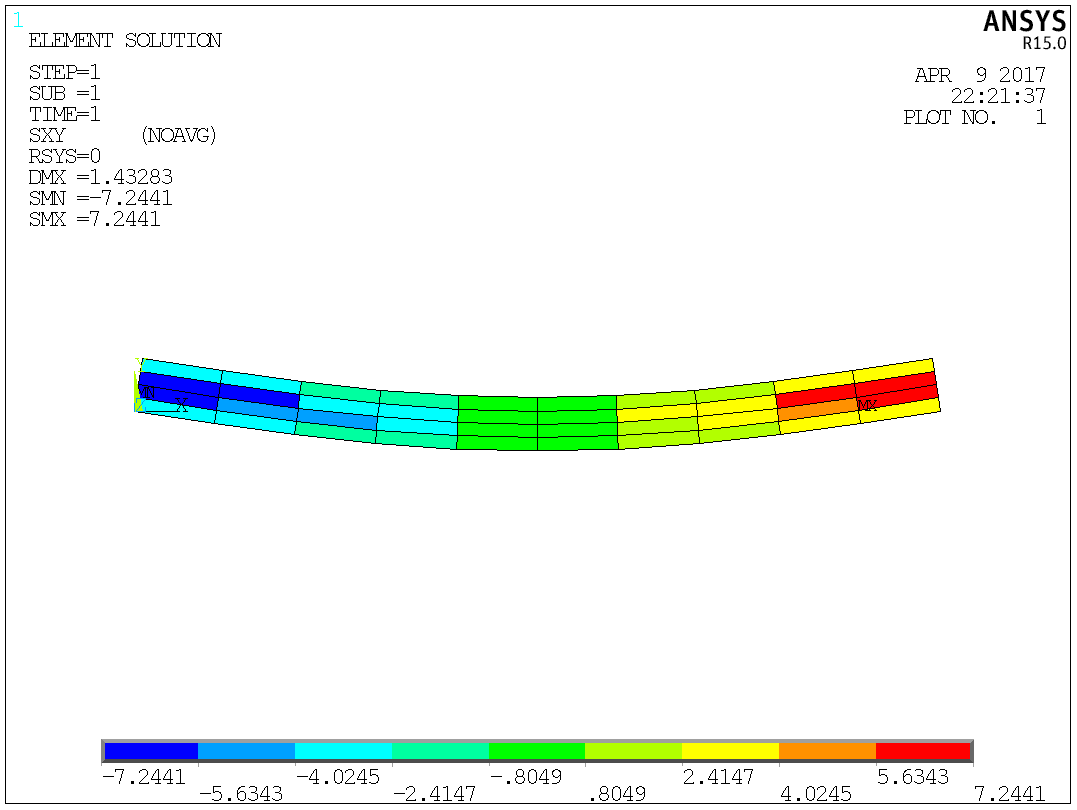
\includegraphics[width=\textwidth]{images/40_SXY}
		\caption{Mapa de tensions tangencials {$\tau_{xy}$}}
		\label{fig:40_SXY}
	\end{subfigure}
	\hfill
	\begin{subfigure}[t]{\imgS}
		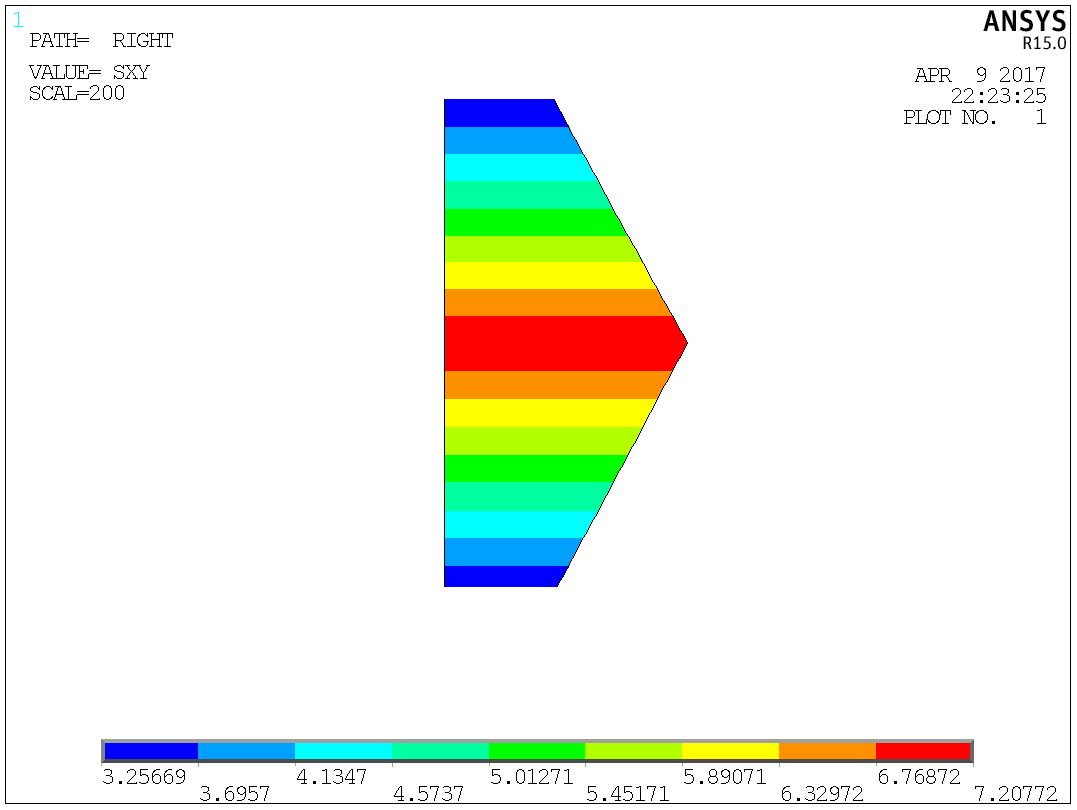
\includegraphics[width=\textwidth]{images/40_SXY_path}
		\caption{Distribució de tensions tangencials a una secció propera a un extrem (\emph{path})}
		\label{fig:40_SXY_path}
	\end{subfigure}
	\caption{Resultats de les tensions tangencials}
	\label{fig:40_shear}
\end{figure}
Les tensions tangencials màximes es troben als extrems de la peça, s'observa un valor de $\tau_{xy,\max+} = 7.24 MPa$ i $\tau_{xy,\max-} = -7.24 MPa$. També es pot observar que per aquest mallat que no és gaire refinat, no és clar que el valor que prenguin els resultats siguin del tot correctes ja que no sembla haver-hi continuïtat entre els elements.

\textbf{Càlcul del coeficient de seguretat de la peça (criteri de Von Mises)}
\begin{figure}[H]
	\centering
	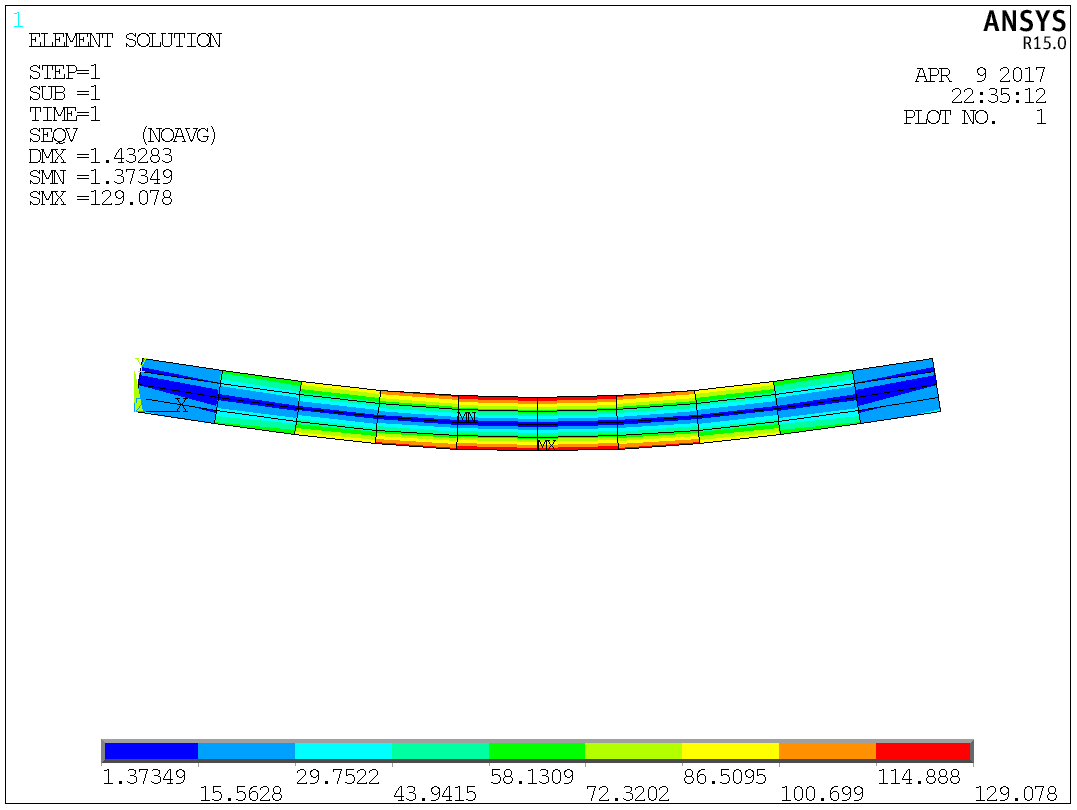
\includegraphics[width=\imgS]{images/40_von_misses}
	\caption{Mapa de tensions equivalents de Von Misses ($\sigma_{eq,VM}$)}
	\label{fig:40_von_misses}
\end{figure}

Donat que s'obté un valor de $\sigma_{eq,VM} = \sigma_{adm} = 129,08$ i que la tensió del límit elàstic és $f_y = 235 MPa$, el coeficient de seguretat serà de $\gamma_{SE} = \frac{f_y}{\sigma_{adm}} = 1,82$.

\pagebreak
\subsection{Anàlisi d'un model amb una malla refinada amb 10 elements en alçada i 40 elements en longitud (10x40 = 400 elements finits)}
\textbf{Anàlisi de la deformada i del desplaçament vertical màxim ($\delta_{y, \max}$)}
\begin{figure}[H]
	\begin{subfigure}{\imgS}
		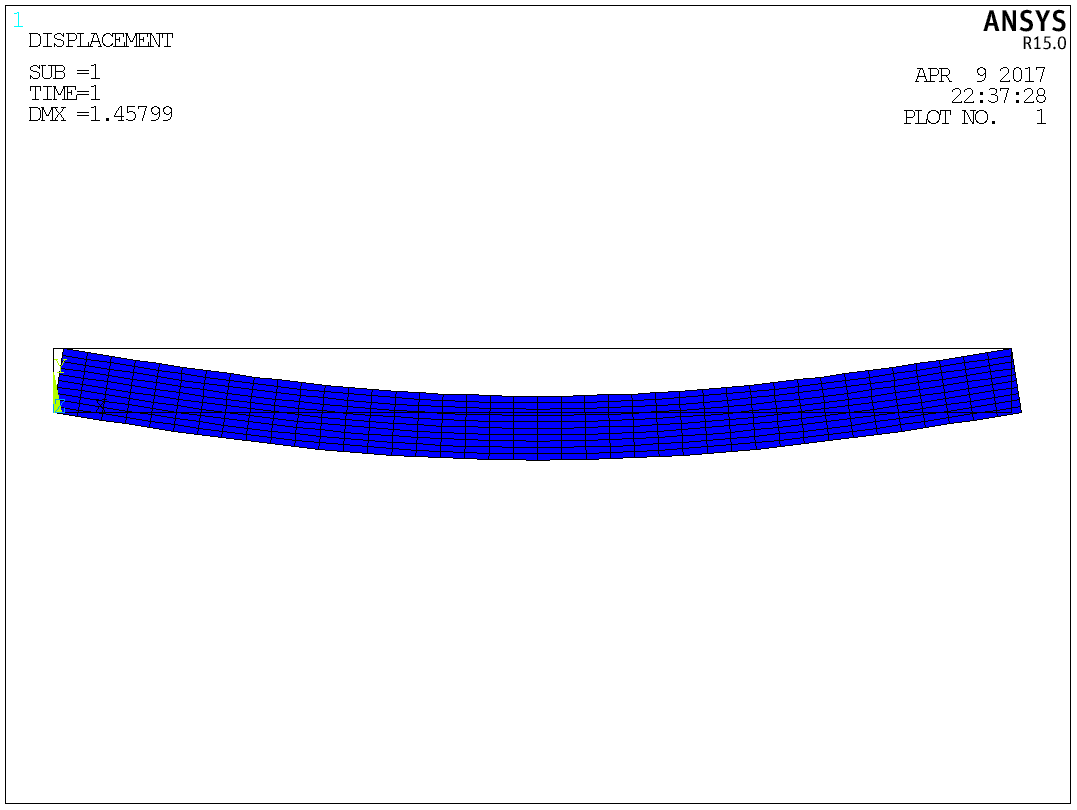
\includegraphics[width=\textwidth]{images/400_deformed}
		\caption{Deformació}
		\label{fig:400_deformed}
	\end{subfigure}
	\hfill
	\begin{subfigure}{\imgS}
		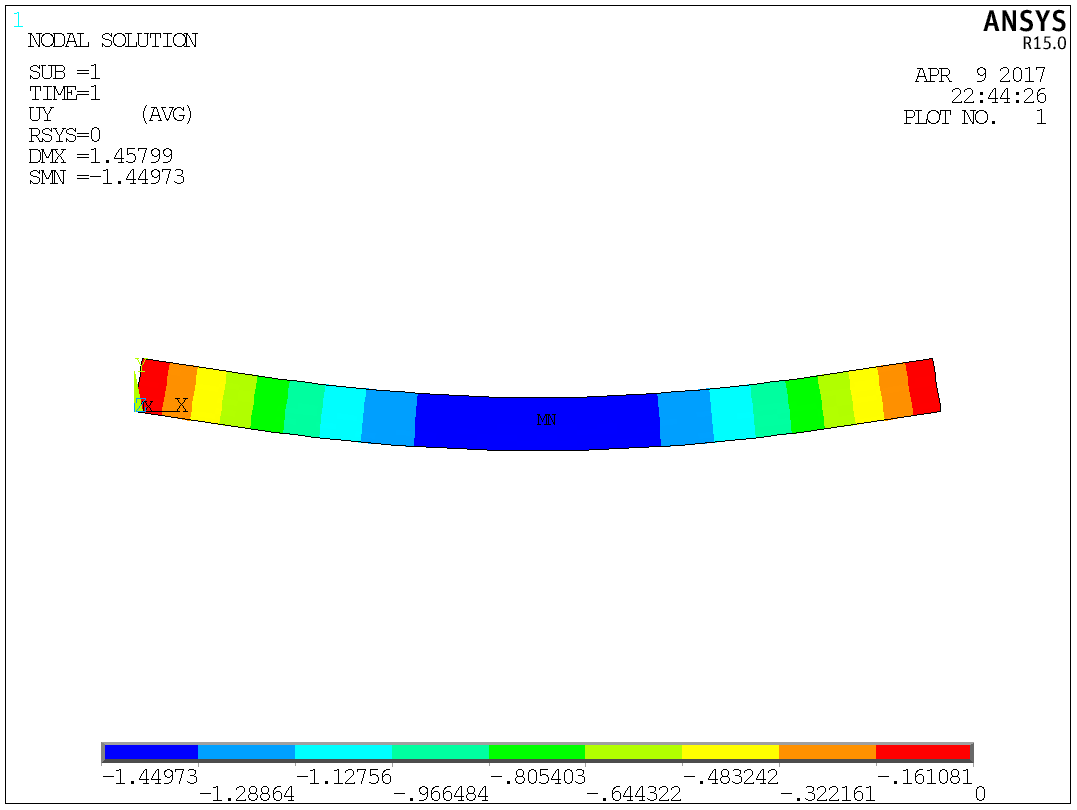
\includegraphics[width=\textwidth]{images/400_UY}
		\caption{Mapa de desplaçaments verticals UY}
		\label{fig:400_UY}
	\end{subfigure}
	\caption{Resultats del desplaçament}
	\label{fig:400_displacement}
\end{figure}
Es pot veure a la \autoref{fig:400_UY} que hi ha un desplaçament màxim $\delta_{y,\max} = 1,45mm$ situat al punt mig de la peça. 

\textbf{Anàlisi de les tensions normals ($\sigma_x$)}
\begin{figure}[H]
	\begin{subfigure}{\imgS}
		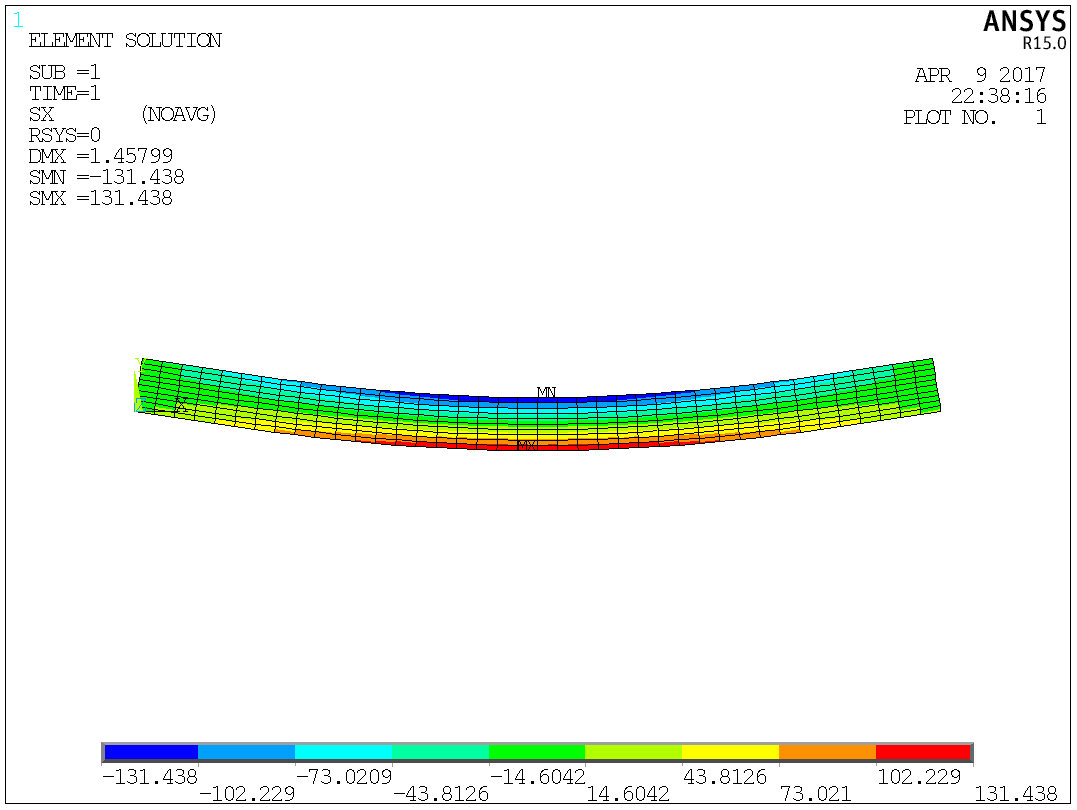
\includegraphics[width=\textwidth]{images/400_stress}
		\caption{Mapa de tensions normals {$\sigma_x$}}
		\label{fig:400_stress}
	\end{subfigure}
	\hfill
	\begin{subfigure}{\imgS}
		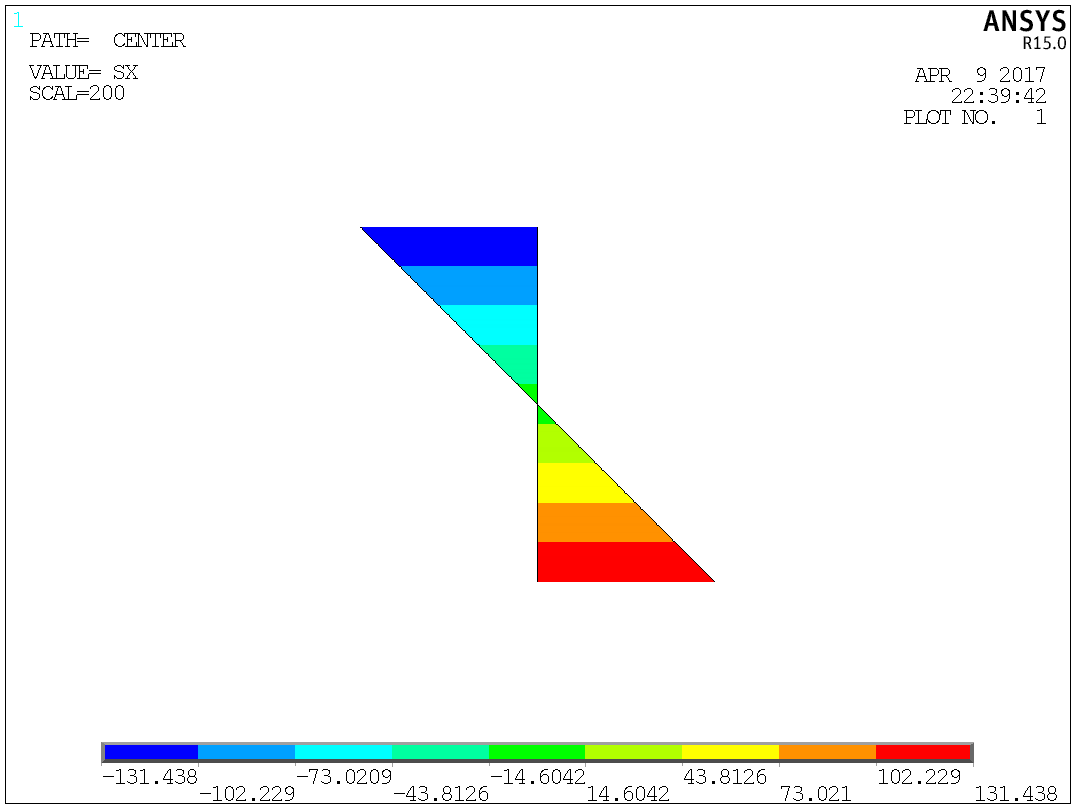
\includegraphics[width=\textwidth]{images/400_stress_path}
		\caption{Distribució de tensions normals a la secció (\emph{path})}
		\label{fig:400_stress_path}
	\end{subfigure}
	\caption{Resultats de les tensions normals}
	\label{fig:400_stress_results}
\end{figure}
Les tensions normals també són màximes al punt mig de la peça, les màximes positives es troben a la part inferior amb valor $\sigma_{x,\max+} = 131,37 MPa$ i les negatives a la part superior amb valor $\sigma_{x,\max-} = -131,37 MPa$. 

\pagebreak
\textbf{Anàlisi de les tensions tangencials ($\tau_{xy}$)}
\begin{figure}[H]
	\begin{subfigure}[t]{\imgS}
		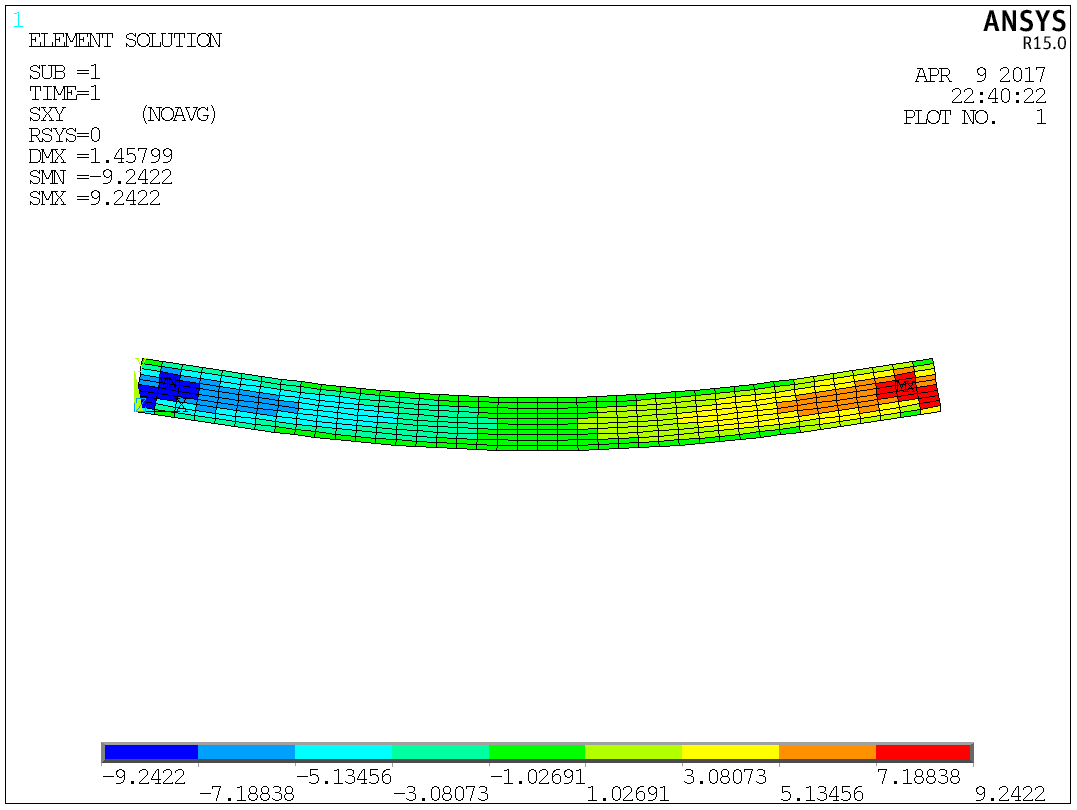
\includegraphics[width=\textwidth]{images/400_SXY}
		\caption{Mapa de tensions tangencials {$\tau_{xy}$}}
		\label{fig:400_SXY}
	\end{subfigure}
	\hfill
	\begin{subfigure}[t]{\imgS}
		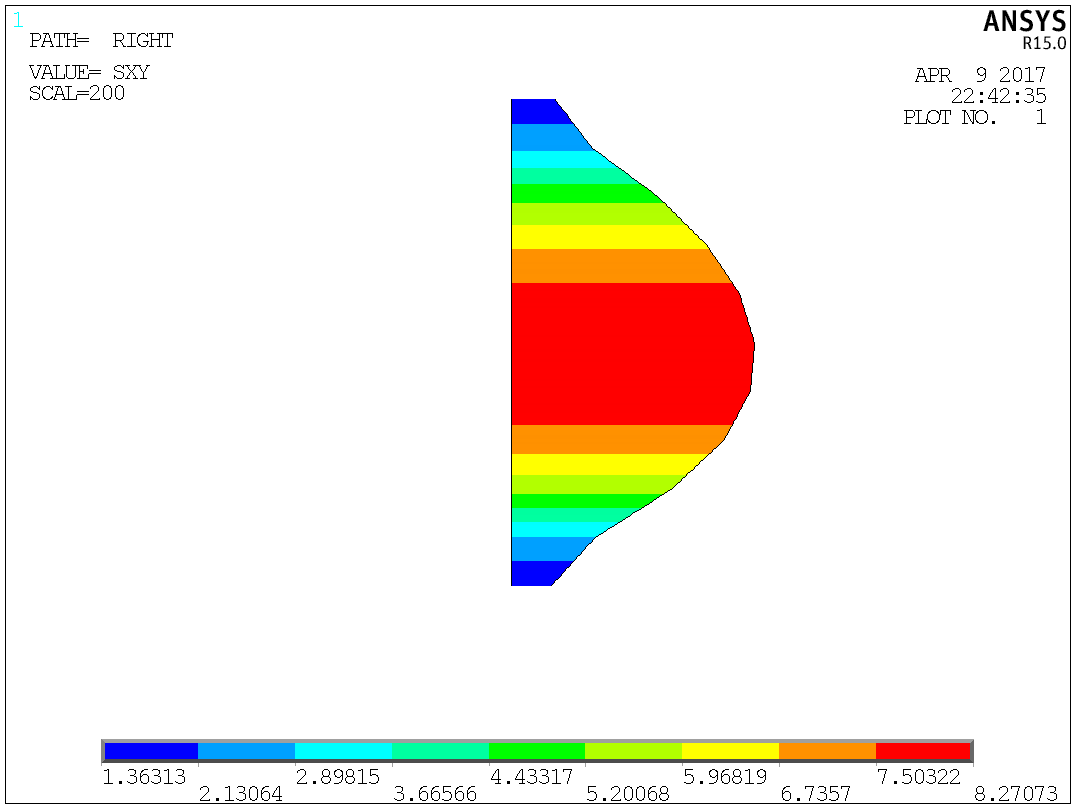
\includegraphics[width=\textwidth]{images/400_SXY_path}
		\caption{Distribució de tensions tangencials a una secció propera a un extrem (\emph{path})}
		\label{fig:400_SXY_path}
	\end{subfigure}
	\caption{Resultats de les tensions tangencials}
	\label{fig:400_shear}
\end{figure}
Les tensions tangencials són màximes als extrems de la peça i prenen valors $\tau_{xy,\max+} = 9,24 MPa$ i $\tau_{xy,\max-} = -9,24 MPa$. En comparació amb el mallat anterior aquí sí que s'observa més continuïtat entre els elements.

\textbf{Càlcul del coeficient de seguretat de la peça (criteri de Von Mises)}
\begin{figure}[H]
	\centering
	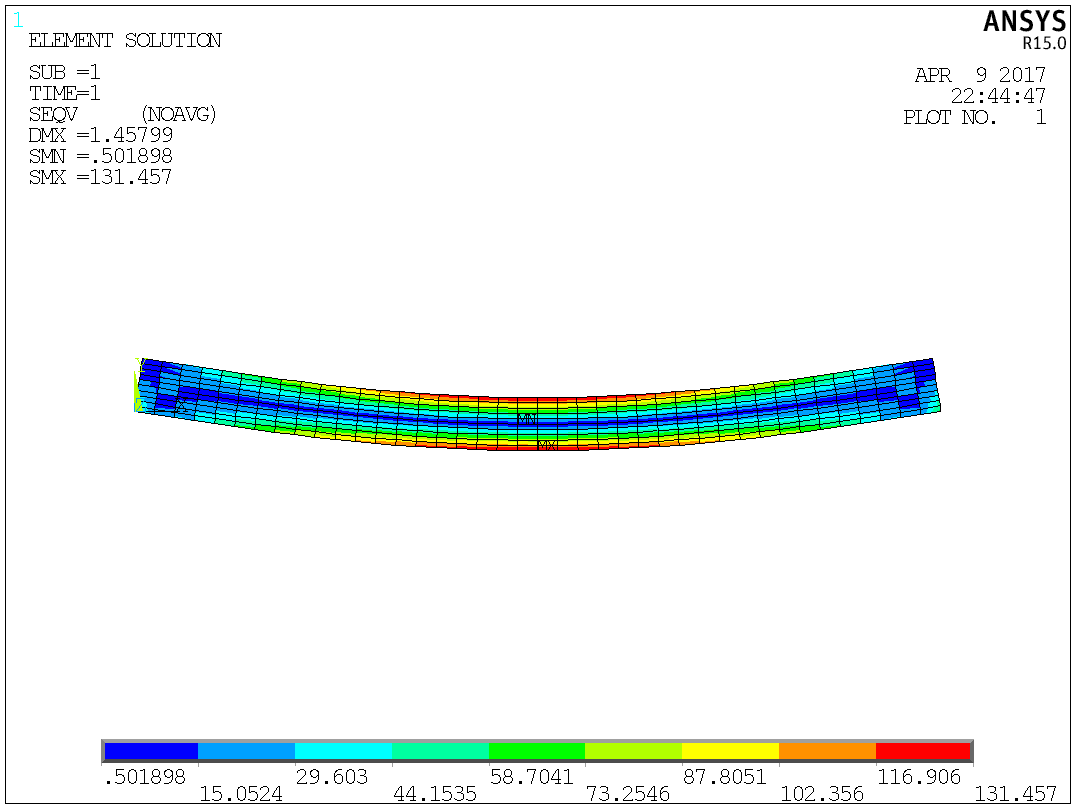
\includegraphics[width=\imgS]{images/400_von_misses}
	\caption{Mapa de tensions equivalents de Von Misses ($\sigma_{eq,VM}$)}
	\label{fig:400_von_misses}
\end{figure}
Donat que el valor màxim de la tensió equivalent de Von Misses és de $\sigma_{eq,VM} = \sigma_{adm} = 131,46 MPa$ i que la tensió del límit elàstic és $f_y = 235 MPa$ el coeficient de seguretat serà $\gamma_{SE} = \frac{f_y}{\sigma_{adm}} = 1,79$.

\subsection{Comparació dels resultats obtinguts amb els resultats teòrics}
\begin{table}[H]
	\centering
	\begin{tabular}{|l|c|r|r|r|}
		\cline{4-5}
		\multicolumn{3}{c|}{\multirow{2}{*}{}} & \textbf{Malla poc refinada} & \textbf{Malla refinada} \\
		\multicolumn{3}{c|}{} & 4x10 = 40 elements & 10x40 = 400 elements \\
		\hline
		\textbf{Paràmetre} & \textbf{Unitats} & \textbf{Solució teòrica} & \textbf{Valor} & \textbf{Valor} \\
		\hline
		$\sigma_{x,\max+}$ & $N/mm^2$ & 133,31 & 128,86 & 131,37 \\
		$\sigma_{x,\max-}$ & $N/mm^2$ & -133,31 & -128,86 & -131,37 \\
		$\tau_{xy,\max+}$ & $N/mm^2$ & 8,88 & 7,2 & 9,24 \\
		$\tau_{xy,\max-}$ & $N/mm^2$ & -8,88 & -7,2 & -9,24 \\
		$\delta_{y,\max}$ & $mm$ & 1,45 & 1,42 & 1,45 \\
		\hline
	\end{tabular}
\end{table}
Es pot observar que els resultats amb la malla refinada són molt més propers a la solució teòrica que els resultats amb la malla poc refinada. En concret, la deformació màxima pren el mateix valor que a la solució teòrica.

\section{Part 2: Simulació amb l'element finit BEAM 188}
\textbf{Anàlisi de la deformada i del desplaçament vertical màxim ($\delta_{y,max}$)}

\begin{figure}[H]
	\begin{subfigure}{\imgS}
		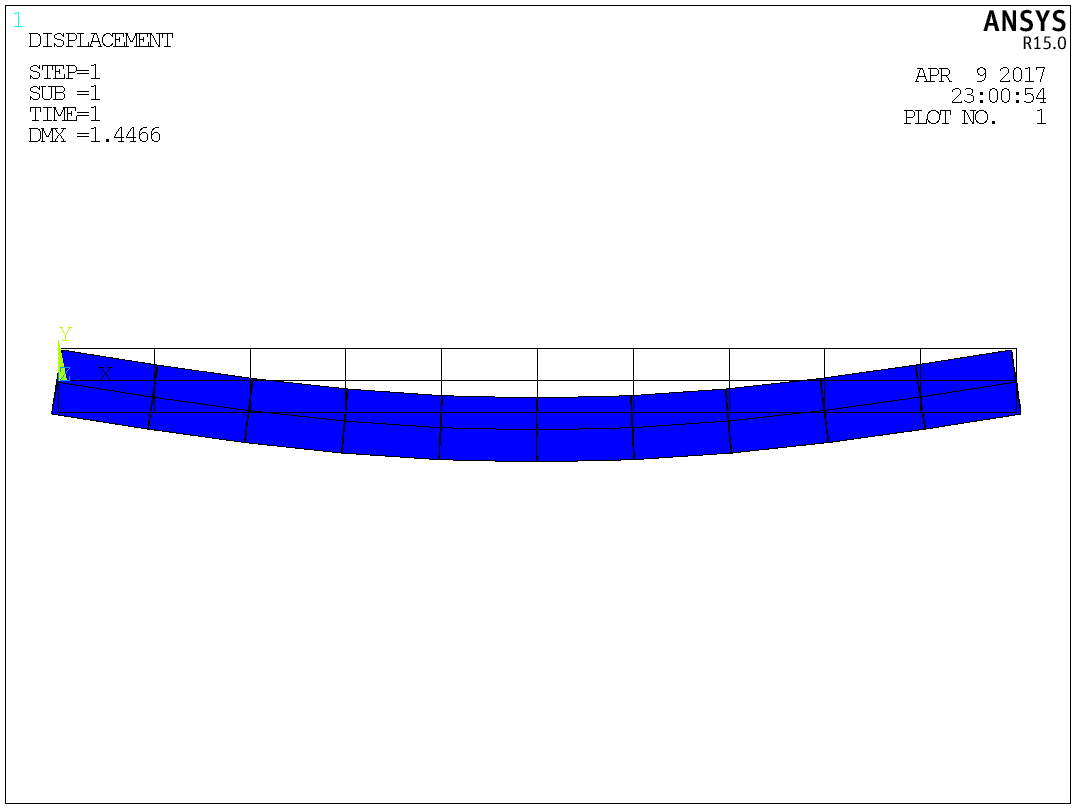
\includegraphics[width=\textwidth]{images/b_deformed}
		\caption{Deformació}
		\label{fig:b_deformed}
	\end{subfigure}
	\hfill
	\begin{subfigure}{\imgS}
		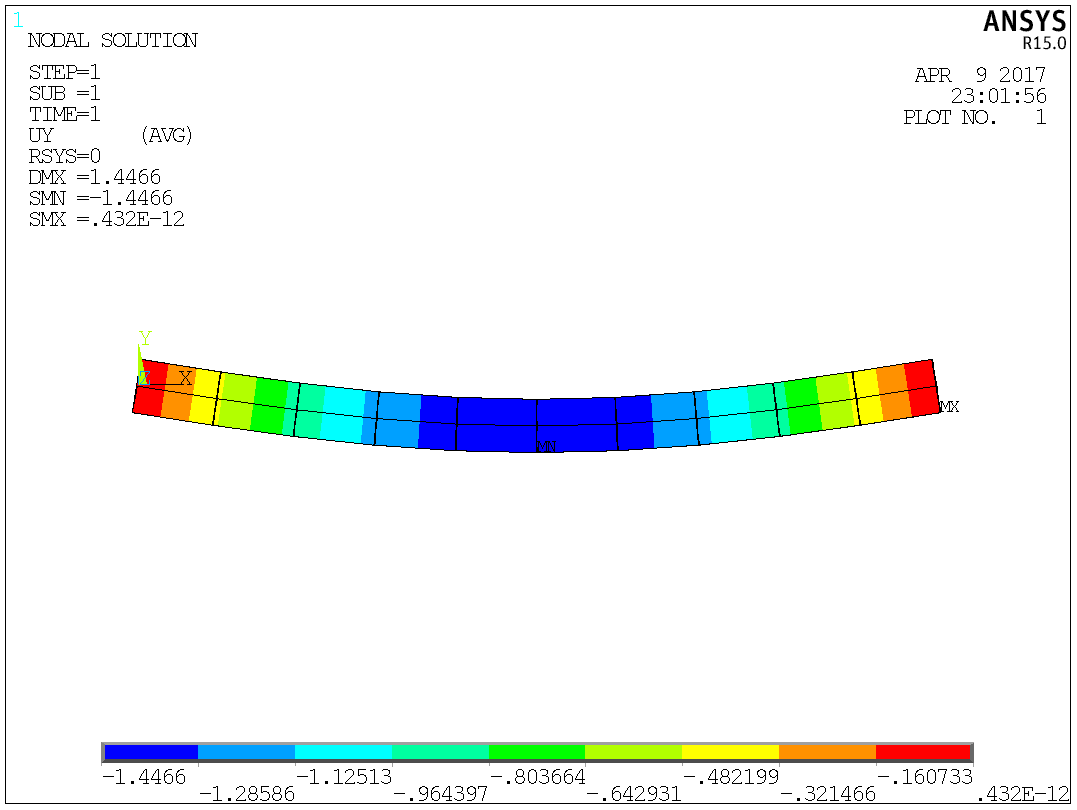
\includegraphics[width=\textwidth]{images/b_UY}
		\caption{Mapa de desplaçaments verticals UY}
		\label{fig:b_UY}
	\end{subfigure}
	\caption{Resultats del desplaçament}
	\label{fig:b_displacement}
\end{figure}
El desplaçament vertical màxim és de $\delta_{y,\max} = -1,45mm$. 

\textbf{Anàlisi del diagrama de moments flectors ($M_z$)}
\begin{figure}[H]
	\begin{subfigure}{\imgS}
		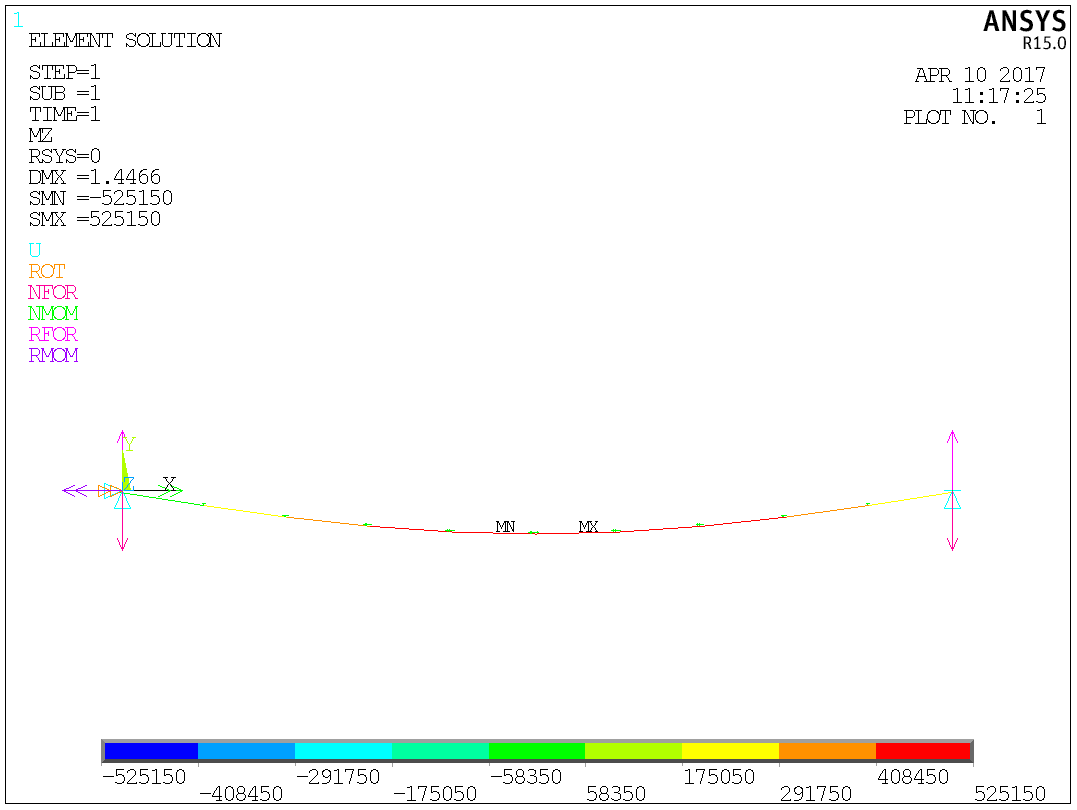
\includegraphics[width=\textwidth]{images/b_MZ}
	\end{subfigure}
	\hfill
	\begin{subfigure}{\imgS}
		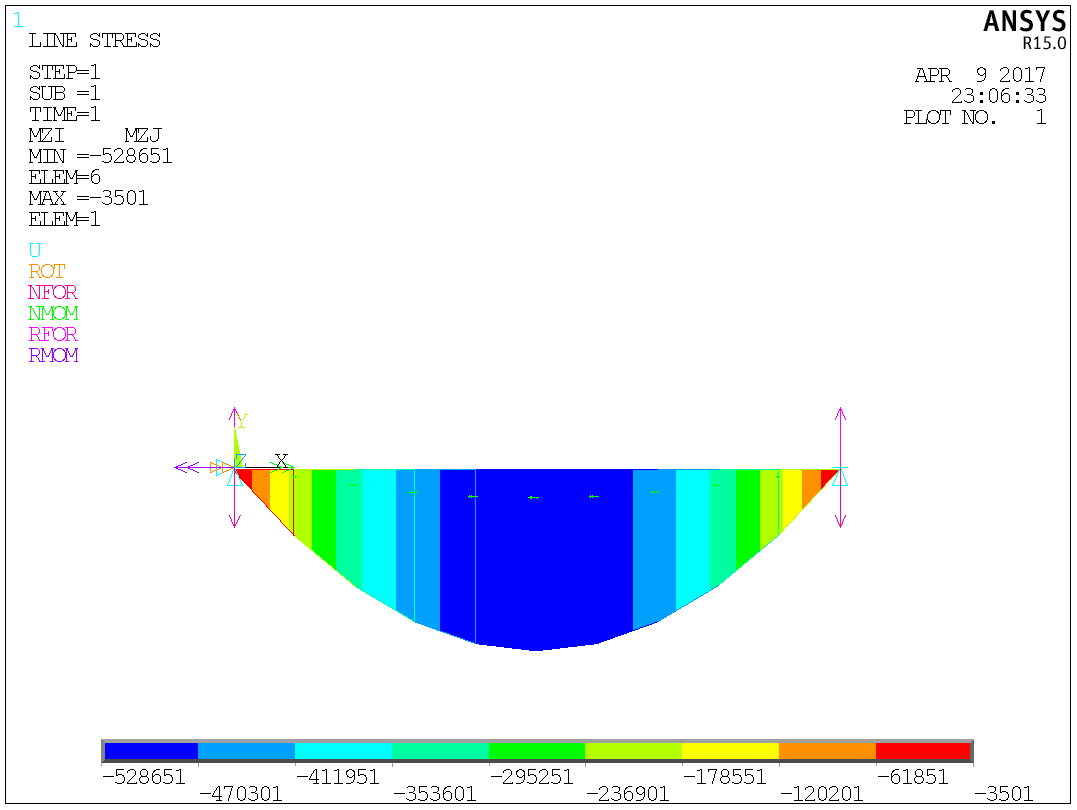
\includegraphics[width=\textwidth]{images/b_MZ_path}
	\end{subfigure}
	\caption{Diagrama de moments flectors $M_z$}
\end{figure}
Pel que fa als moments flectors es pot veure que segueixen una funció quadràtica amb punt màxim al centre i valor $M_{z,\max} = 525,15 N\cdot m$.

\textbf{Anàlisi del diagrama d'esforços tallants ($T_y$)}
\begin{figure}[H]
	\begin{subfigure}{\imgS}
		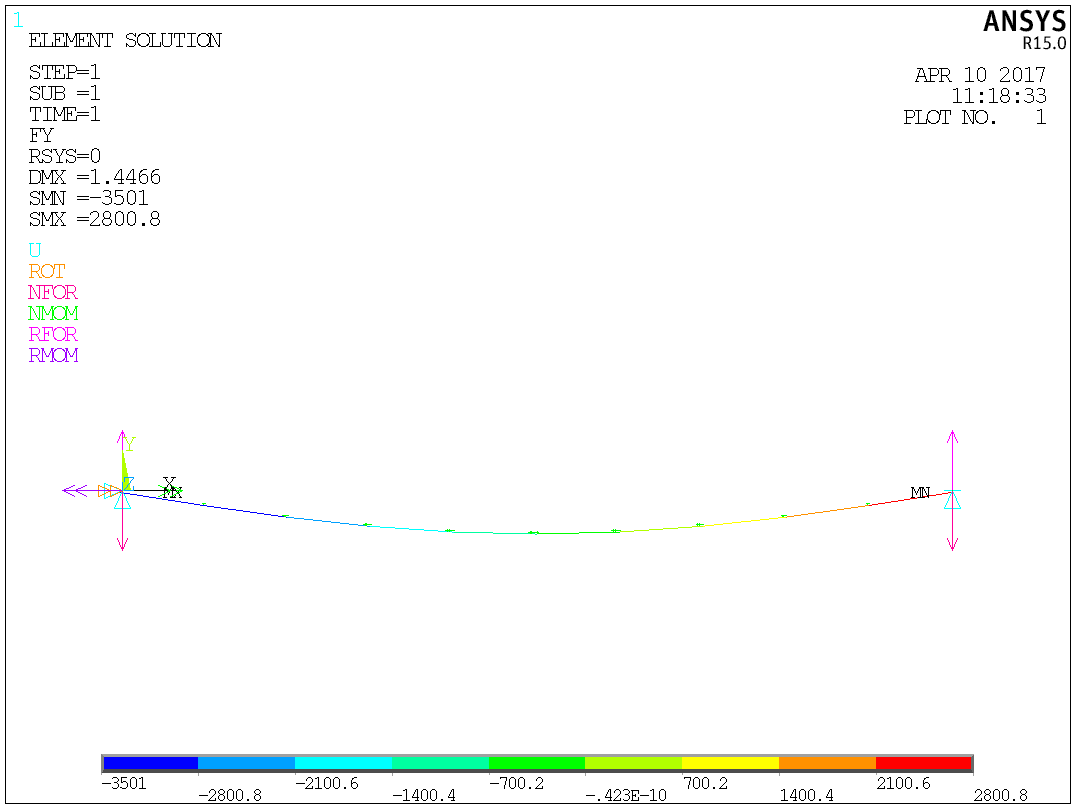
\includegraphics[width=\textwidth]{images/b_TY}
	\end{subfigure}
	\hfill
	\begin{subfigure}{\imgS}
		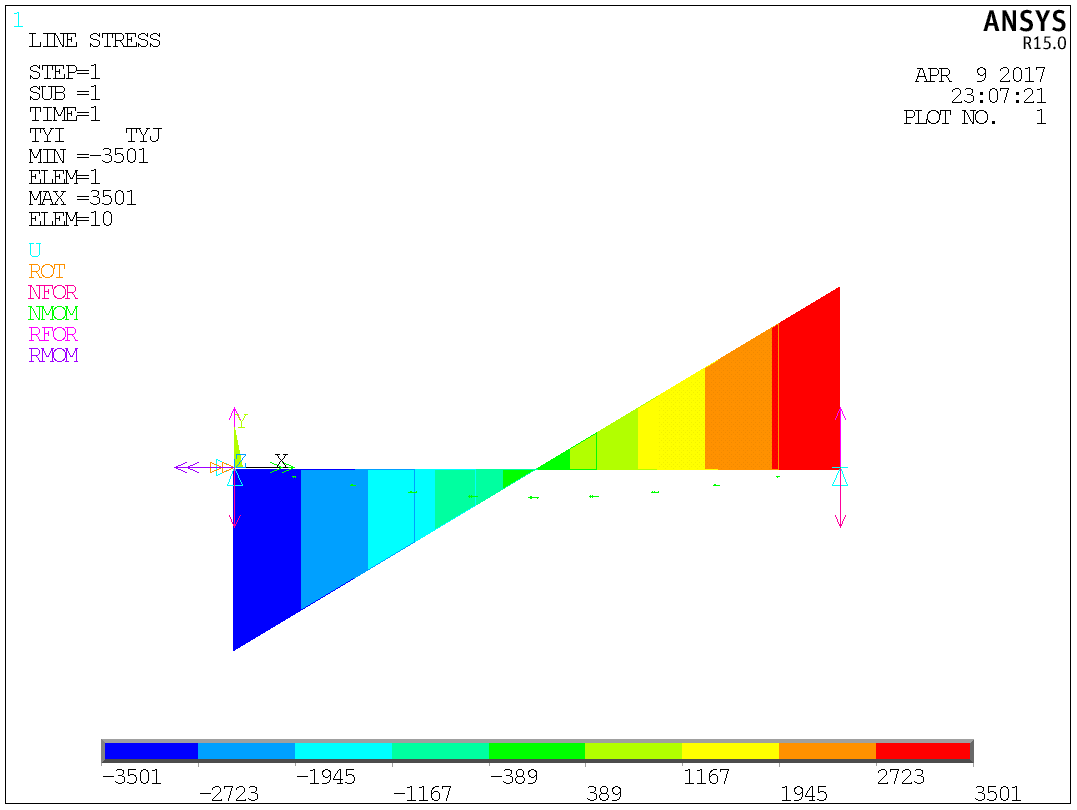
\includegraphics[width=\textwidth]{images/b_TY_path}
	\end{subfigure}
	\caption{Diagrama d'esforços tallants $T_y$}
\end{figure}
Els esforços tallants són màxims als extrems i neutres al punt mig.

\section{Part 3: Expressar l'estat de tensió a un punt crític de la peça}
\subsection{Determinar el tensor tensió a un punt crític de la tensió}

Per a la resolució d'aquesta qüestió, s'han considerat els resultats del model amb malla refinada (400 elements). S'ha analitzat la secció crítica (centre de la peça) i en concret el punt situat a una distància $y=-\frac{h}{2}$ de l'eix neutre.
\begin{figure}[H]
	\centering
	\begin{tikzpicture}
		\draw[dashed, gray] (-1.5, 0) -- (1.5, 0) node[at start, anchor = east, black]{z};
		\draw[dashed, gray] (0, -2.25) -- (0, 2.25) node[black]{y};
		\draw[pattern = north east lines, pattern color = gray] (-.75, -2) rectangle (.75, 2);
		\dimline[extension start length=-1.25cm,
			extension end length=-.5cm,
			extension start style={black, thin},
			extension end   style={black, thin},
		]{(2, -2)}{(2, 0)}{$y=-\frac{h}{2}$};
		\dimline[extension start length=-2.25cm,
			extension end length=-2.25cm,
			extension start style={black, thin},
			extension end   style={black, thin},
		]{(3, -2)}{(3, 2)}{$h=40mm$};
		\dimline[extension start length=-1cm,
			extension end length=-1cm,
			extension start style={black, thin},
			extension end   style={black, thin},
			label style={below=0.8ex}
		]{(-.75, -3)}{(.75, -3)}{$b=15mm$};
		\fill (0, -2) circle[radius=2pt];
	\end{tikzpicture}
\end{figure}

Els components del tensor tensió $\sigma_y$, $\sigma_z$ i $\tau_{xy}$ són nuls d'acord amb les hipòtesis de peça prismàtica pel que el tensor tensió final és:
$$
\left[\sigma\right]_{x,y,z,\text{punt 1}} = 
\begin{bmatrix}
\sigma_x & \tau_{xy} & \tau_{xz} \\
\tau_{xy} & 0 & 0 \\
\tau_{xz} & 0 & 0
\end{bmatrix} = 
\begin{bmatrix}
131,37 & -6,32\cdot 10^{-11} & 0 \\
-6,32\cdot 10^{-11} & 0 & 0 \\
0 & 0 & 0
\end{bmatrix}
$$

\section{Conclusions}
Gràcies a la realització d'aquesta practica hem pogut veure les diferencies entre el model que utilitzem de barra a teoria  i el model de elements finits. També ens ha permès veure a diferencia entre diferents mallats així com repassar diferents criteris de ruptura i respectius coeficients de seguretat.
\end{document}